\chapter{Testing}
\renewcommand{\baselinestretch}{\mystretch}
\label{chap:Testing}
\section{Overview}
%\setlength{\parindent}{0pt}
The testing of this system split into a logical correctness test; using multiple tools to identify any errors in the execution of the system, and a robust resource utilisation test. A number of tests with different parameters will be introduced in the testing section with their results shown in tables and figures below. Each of these tests will then be discussed in the evaluation section comparing the solution to the benchmark code that runs in simulation provided at the start of the report as well as other solutions that were discussed in the related work section. 

\section{Logical Verification}
The original comparison engine was made available as the basis for this project written in hardware description language VHDL, it works fully running under simulation in Modelsim. For the purposes of this project that code is used as a golden standard and later as a benchmark. Any bit error inconsistencies in the results are treated as errors. The design of this project was specifically organised such that there should be bit-wise consistency between the provided code and the implemented solution. It is important to note however, there are some limitations on this with regards to the non-deterministic effects introduced by clock skew across multiple devices and data transfer errors. Test data is inserted to both the simulation and the hardware implementation, both results are written out to text files in the same format. This text file is then checked for binary equality. 


A MATLAB version of the algorithm was also made available, however this produces different bitwise results, measuring the integer distance in overlaps rather than the bit-distance. As a result this was not suitable for verification. 


The full testing procedure consisted of varying several parameters, fitting from 5 to 12 pixels per device, testing read lengths of up to 1000 base pairs and changing the local library parameters to control the level of sensitivity the comparison engine. Having fully tested the FPGA based implementation it was found to produce correct results under the following set of test conditions. 

\begin{table}[!h]
\centering % used for centering table
\begin{tabular}{c c c c c c} % centered columns (4 columns)
\hline\hline %inserts double horizontal lines
Read Length & Genome Length & Pixel Count & FPGA Count & Library Size & Correct\\ [0.5ex] % inserts table 
%heading
\hline % inserts single horizontal line
50 & 113 & 5 & 1 & 5 & Yes \\ % inserting body of the table
400 & 1500 & 9 & 1 & 5 & Yes \\% [1ex] adds vertical space
400 & 3000 & 27 & 3 & 5 & Yes \\% [1ex] adds vertical space
400 & 3000 & 27 & 3 & 3 & Yes \\% [1ex] adds vertical space
400 & 3000 & 27 & 3 & 10 & Yes \\% [1ex] adds vertical space
1000 & 2000 & 20 & 2 & 10 & Yes \\% [1ex] adds vertical space
1000 & 10000 & 36 & 3 & 10 & Yes \\% [1ex] adds vertical space
\hline
\end{tabular}
\caption{Validation Results} % title of Table
\label{table:nonlin}
\end{table}


All parameters not listed were set as default as listed in appendix \ref{App:default}. 



\section{Performance Characteristics}
\subsection{Resource Usage}
The performance characteristics of the comparison engine can be measured in different metrics, all of which have significant practical meanings; logic utilisation, memory utilisation, clock frequency, and cycle count. A derived measurement of cumulative speed will also be shown, derived from the clock speed and cycle count measurements.

\subsubsection{Logic Utilisation}

Logic utilisation measures how much of the FPGA device is used by a given circuit and in the case of the comparison engine, is the limiting factor for how many pixels can fit on a single device. This measurement will be compared to the simulated implementation (referred to as the benchmark) in order to show how all of the data communication and control logic has increased the design. The ideal for this metric is to keep the logic utilisation as low as possible. In order to draw this comparison a number of parameters will be changed and the logic utilisation recorded. Ordinarily, due to the size of the FPGA this comparison would be very limited as the provided code would only work on a single device, in order to draw a good comparison of logic utilisation at the same computational level, a larger FPGA based on the same technology will be used for comparison. A discussion of the true achievable computational power will follow later. The full set of results are listed in \ref{table:logic}. For these tests identical compilation settings were used to guarantee the comparison were valid, and Altera CYCLONE III devices were used.

As a separate analysis of the resource utilisation, figure \ref{table:single} shows a break down of the resource utilisation of each sub-block. This shows the IO controller, built as part of this project's implementation uses around 2,700 logic elements, this translates to around 1-2 pixels worth of logic. This is cost of being able to scale across multiple FPGAs. Effectively the area available for pixels on the DE0 device is reduced by 2,700 logic elements but multiple FPGA's space becomes available. To further quantify this, the logic usage of various numbers of pixels was plotted. This is shown in figure \ref{fig:fpgacount}, it shows that the control logic introduces around a 1,000 logic element overhead for small pixel counts. At the larger pixel count, routing had a significant effect and the interconnection of the control logic caused bad scaling in the routing.



\begin{table}[!h]
\centering % used for centering table
\begin{tabular}{c c} % centered columns (4 columns)
\hline %inserts double horizontal lines
\hline
Sub-Block & Logic Elements\\  % inserts table 
\hline
Global Controller & 158 \\
Pixel Array & 12,047 \\
IO Controller & 2,272 \\
Scheduler & 192 \\
UART & 85\\
%heading
\hline
\end{tabular}
\caption{Resource Utilisation of a single Master processor with 9 pixels} % title of Table
\label{table:single}
\end{table}


\subsubsection{Memory Utilisation}
Similarly to logic utilisation, memory utilisation measures how much of the device resources are used by the design. As covered in the analysis of Y Hu's comparison engine, memory utilisation was very low for this algorithm. For this reason less importance was placed on minimising its usage. To quantify this, when over 80\% of a device's logic was used, less than 1\% of the onboard memory was used. The memory utilisation is affected by a sub-set of the parameters, read length, pixel count, and library size. These parameters set the size of the local FIFO buffers. The main priority with memory utilisation is only to ensure that the memory doesn't not scale significantly worse than the logic element utilisation. This will be discussed later in the evaluation section.


\vspace*{\fill}


\begin{sidewaystable}[p]
\centering % used for centering table
\begin{tabulary}{\textwidth}{C C C C| C C| C C C C}% centered columns (4 columns)
\hline\hline %inserts double horizontal lines
Read Length & Genome Length & Pixel Count & Library Size & Benchmark Logic Elements & Benchmark Memory Bits & Cluster Size & Implementation Logic Elements & Implementation Memory Bits \\
\hline 
% inserts single horizontal line
50 & 113 & 9 & 5 & 10,608 & 4,096 & 3 & (5,808)~(5,175) & (5,620)~(4,532)\\
50 & 113 & 15 & 5 & 17,564 & 4,096 & 3 & (7,946)~(8,230) & (6,612)~(4,732)\\
50 & 113 & 27 & 5 & 31,697 & 4,096 & 3 & (14,097)~(14,021) & (8,908)~(5,140)\\
50 & 113 & 45 & 5 & 54,342 & 4,096 & 3 & (21,701)~(26,448) & (12,124)~(5,740)\\
50 & 113 & 99 & 5 & 116,496 & 4,096 & 3 & (44,825)~(48,578) & (22,732)~(7,548)\\
\hline
50 & 100 & 27 & 5 & 31,697 & 4,096 & 3 & (14,097)~(14,021) & (8,908)~(5,140)\\
50 & 1,000 & 27 & 5 & 31,697 & 4,096 & 3 & (14,097)~(14,021) & (8,908)~(5,140)\\
50 & 10,000 & 27 & 5 & 31,697 & 4,096 & 3 & (14,097)~(14,021) & (8,908)~(5,140)\\
\hline
50 & 2,000 & 27 & 5 & 31,697 & 4,096 & 3 & (13,404)~(14,021) & (8,908)~(5,140)\\
100 & 2,000 & 27 & 5 & 31,936 & 4,096 & 3 & (13,290)~(14,065) & (9,952)~(6,048)\\
200 & 2,000 & 27 & 5 & 32,191 & 4,096 & 3 & (13,448)~(14,045) & (11,872)~(7,848)\\
400 & 2,000 & 27 & 5 & 32,276 & 4,096 & 3 & (13,400)~(14,082) & (15,616)~(11,456)\\
800 & 2,000 & 27 & 5 & 32,604 & 4,096 & 3 & (14,122)~(14,593) & (22,960)~(18,664)\\
1,600 & 2,000 & 27 & 5 & 32,716 & 4,096 & 3 & (14,253)~(14,584) & (37,360)~(33,064)\\
\hline
50 & 400 & 27 & 3 & 29,490 & 4,096 & 3 & (13,341)~(12,967) & (7,348)~(5,084)\\
50 & 400 & 27 & 5 & 30,747 & 4,096 & 3 & (13,404)~(13,828) & (8,908)~(5,140)\\
50 & 400 & 27 & 10 & 37,165 & 4,096 & 3 & (16,212)~(16,151) & (12,820)~(5,284)\\
50 & 400 & 27 & 20 & 47,831 & 4,096 & 3 & (20,891)~(20,116) & (20,668)~(5,580)\\
\hline 
50 & 400 & 40 & 5 & 50,513 & 4,096 & 1 & (58,609)~(N/A)~~~ & (13,896)~(N/A)\\
50 & 400 & 40 & 5 & 50,513 & 4,096 & 2 & (28,284)~(26,957) & (11,904)~(6,240)\\
50 & 400 & 40 & 5 & 50,513 & 4,096 & 4 & (15,084)~(14,116) & (10,888)~(5,240)\\
50 & 400 & 40 & 5 & 50,513 & 4,096 & 5 & (12,623)~(10,931) & (10,696)~(5,040)\\
50 & 400 & 40 & 5 & 50,513 & 4,096 & 8 & (8,799)~(7,735) & (10,420)~(4,740)\\
50 & 400 & 40 & 5 & 50,513 & 4,096 & 10 & (7,442)~(5,958) & (10,336)~(4,640)\\
\hline
\end{tabulary}
\caption{Comparison of Logic Utilisation, Implementation listed as (Master)(Each Slave)} % title of Table
\label{table:logic}
\end{sidewaystable}

\begin{figure}[p]
  \centering
  \includegraphics[height=0.4\textheight]{./figs/eps/fpga_count.pdf}
  \caption{Resource Utilisation Scaling with Device Count}
    \label{fig:fpgacount}
\end{figure}
\begin{figure}[p]
  \centering
  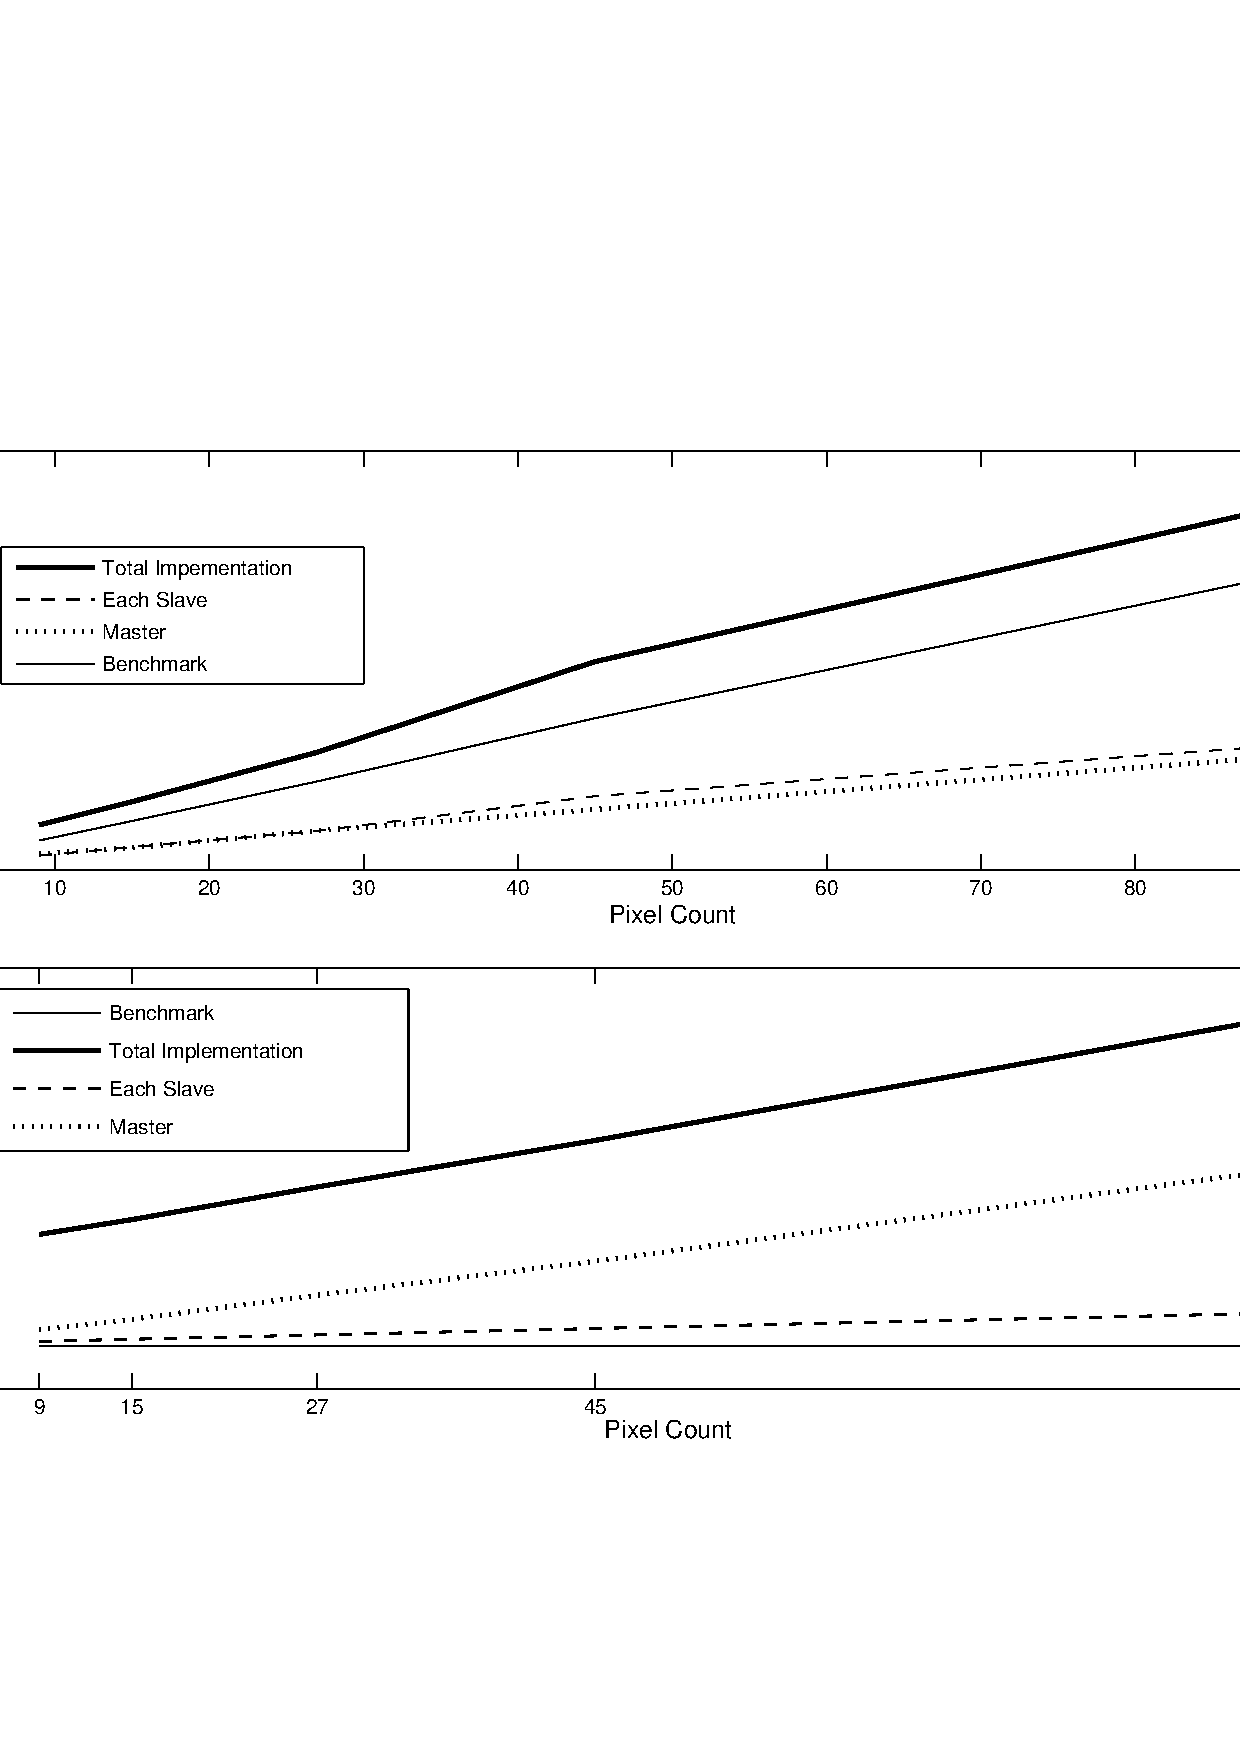
\includegraphics[height=0.4\textheight]{./figs/eps/pix.pdf}
  \caption{Resource Utilisation Scaling with Pixel Count}
    \label{fig:pix}
\end{figure}
\begin{figure}[p]
  \centering
  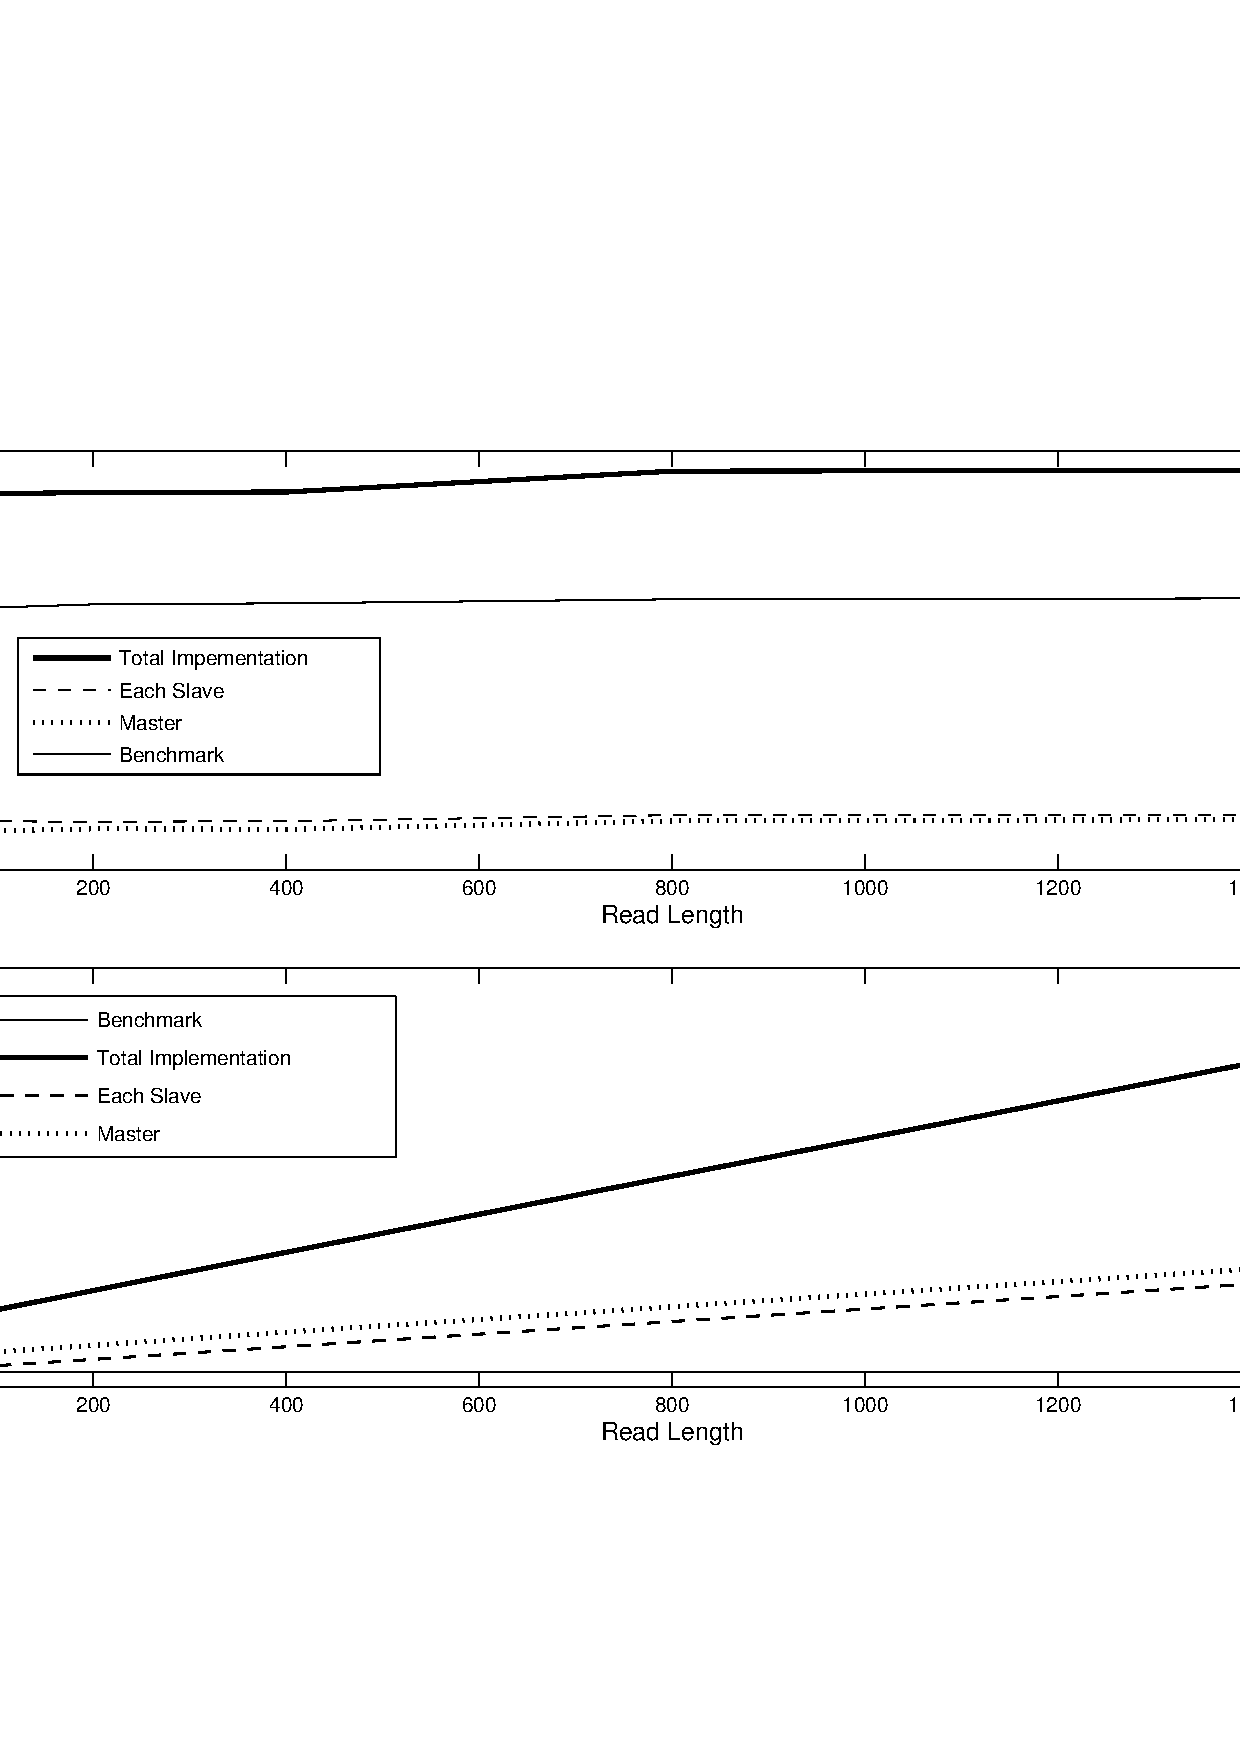
\includegraphics[height=0.4\textheight]{./figs/eps/read_length.pdf}
  \caption{Resource Utilisation Scaling with Read Length}
    \label{fig:read}
\end{figure}

\begin{figure}[p]
  \centering
  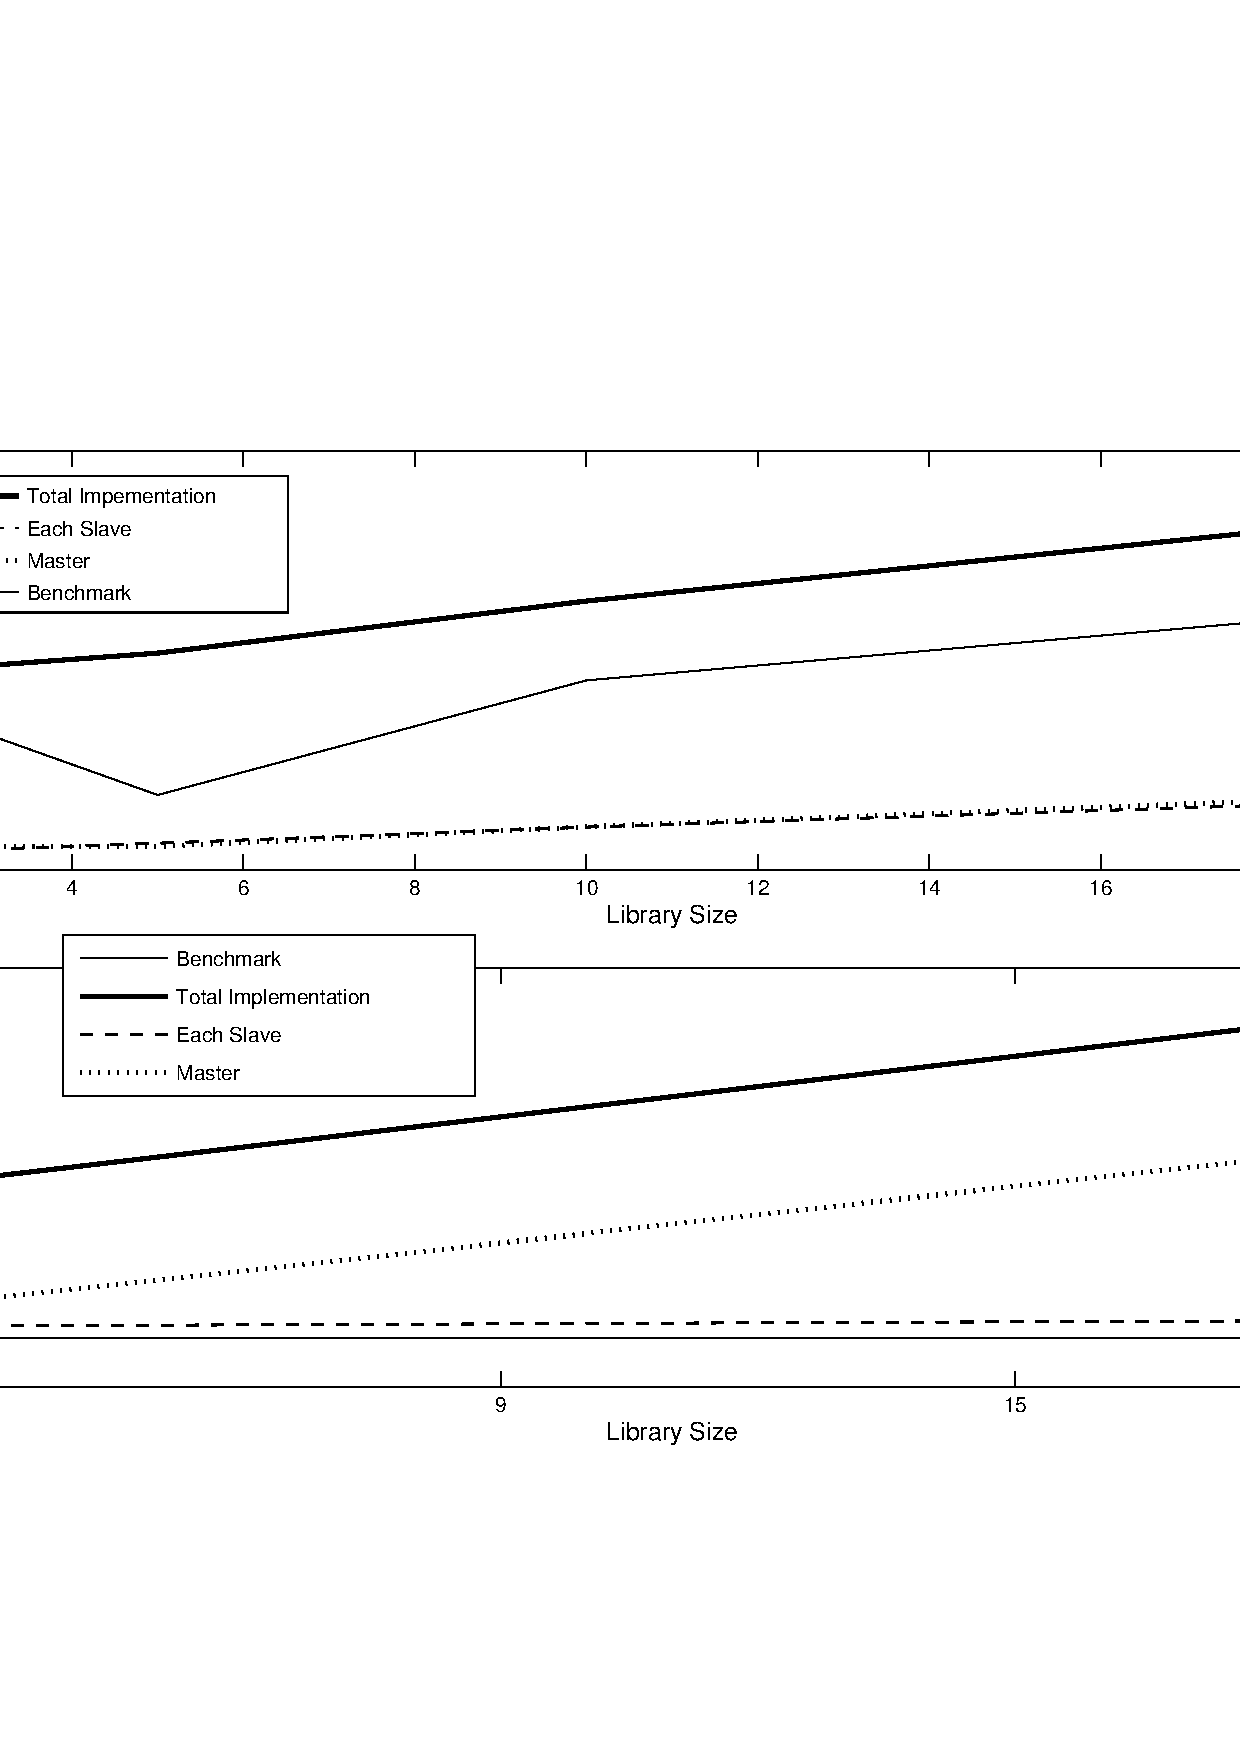
\includegraphics[height=0.4\textheight]{./figs/eps/lib_size.pdf}
  \caption{Resource Utilisation Scaling with Library Size}
    \label{fig:lib}
\end{figure}

\pagebreak
\subsection{Speed}
\subsubsection{Clock Frequency}
Clock frequency is one part of the equation for determining how fast the comparison engine can produce results. In the background section the clock speed of a single pixel was measured within the context of the process. Individually a pixel can reach 40.6~MHz, however within any full design drops to 33.1~MHz. In the implementation section however, more limitations were discussed for clock speed, due to the relatively long wiring between FGPAs and the shared clock domain. Within the calculations there a theoretical 260MHz could be reached, which far surpasses the local limitations. In this section the clock speed will be increased from 1~MHz to a full 33~MHz in practical tests and any bit errors in the results will be noted.



\subsection{Cycle Count}
Cycle count is a term which refers to how many clock cycles are required for a full comparison cycle between pieces of a string to happen. In the case of this algorithm there is a new comparison cycle after each new piece of pixel data arrives. This algorithm consists of two stages, the first where data is clocked in and buffers are filled, and the second where the buffers are filled and pixels are forwarding data. This second stage is the vast majority of the  processing time of the algorithm and therefore is the most important part to measure. In order to count the number of cycles, simulation data will be used, as measuring a single comparison cycle on the device is practically impossible. The way the algorithm executes is such that the cycle counts in simulation and on device should be identical. This data is shown in figure \ref{fig:wave}. This simulation was conducted as a comparison between 9 pixels in the benchmark code, and 9 pixels split across 3 devices on the 25th comparison cycle of a 50 read length sub-sequence.

\begin{sidewaysfigure}[!h]
  \centering
  \includegraphics[width=\textheight]{./figs/provided.png} 
  \vspace*{4em}
 
   \includegraphics[width=\textheight]{./figs/MFPGA.png}
  \caption{Single Comparison Cycle. Left: Single FPGA Simulation; 29 Clock Cycles per Comparison Cycle. Right: 3 FPGA Cluster Simulation; 35 Clock Cycles per Comparison Cycle}
  \label{fig:wave}
\end{sidewaysfigure}

\subsection{Cumulative Speed}
As well as measuring the achieved frequency and the cycle count, it is important to look at the total speed of the algorithm. This can be done in two ways, the first is measuring the core speed of the algorithm, using the data provided by the clock frequency and cycle count. The second is to measure the total time between sending data to the hardware accelerator and receiving the full result library. The first can be done analytically with the data collected in the previous subsections; the time per comparison versus the clock speed.

\begin{align*}
\text{Comparison Rate} &= \frac{\text{Comparisons in Parallel} \times \text{Clock Frequency}}{\text{Cycles per Comparison}} \\
&= \frac{27\times 31\times 10^6}{35} \\
&= 23~\text{Million Comparisons per Second}
\end{align*}

One comparison occurs for each element of the string, and so for a 50 read length sample, 478 000 comparisons per second can be achieved. It is important to note though, this is only theoretical throughput. Data communication with the FPGA is a significant portion of the time, and this is best measured through practical testing. 


These practical tests can be carried out by using timers in the python host software to measure and report the time taken to do the full comparison and read out results. This takes into account all possible causes of delay and gives a much more accurate picture of the processing speed of the algorithm on this specific cluster.

This testing was done by sending overlap data to the device and receiving the result data 5 times within a timing section. The time measured was then divided by 5 to get the speed of a single set of comparisons. Various read lengths were run in order to see the effect of scaling the pixels to longer problems. 

The results of this test are listed in figure \ref{table:speed} with a pixel count of 27, and FPGA count of 3.  In order to minimise the impact of noise each measurement is an average of 10 runs of the algorithm, due to the nature of the program there should be no initial run cost. Only the comparison is being measured for speed, any data translations on the host side are not accounted for as in a full tool-chain these would vary significantly.


\begin{table}[!h]
\centering % used for centering table
\begin{tabular}{c c c c c c} % centered columns (4 columns)
\hline\hline %inserts double horizontal lines
Read Length & Genome Length & Library Size & Time (ms)\\ [0.5ex] % inserts table 
%heading
\hline % inserts single horizontal line
25 & 600 & 5 & 25\\ % inserting body of the table
50 & 600 & 5 & 31\\ % inserting body of the table
75 & 600 & 5 & 43\\ % inserting body of the table
100 & 600 & 5 & 59\\ % inserting body of the table
200 & 600 & 5 & 123\\ % inserting body of the table
400 & 600 & 5 & 229\\ % inserting body of the table
\hline
\end{tabular}
\caption{Practical Speed Tests} % title of Table
\label{table:speed}
\end{table}



